\section{Результаты численных экспериментов}
Вычислительные эксперименты проводились на узле суперкомпьютера «Лобачевский», установленного в ННГУ им. Н.И. Лобачевского, на сегменте под управлением операционной системы семейства Windows (HPC Server 2008). Узел располагает двумя процессорами Intel Sandy Bridge E5-2660 2.2 GHz, 64 Gb RAM, и двумя сопроцессорами Intel Xeon Phi 5110P.
\par
В работе \cite{gklsPaper} описан GKLS-генератор, позволяющий порождать задачи многоэкстремальной оптимизации с заранее известными свойствами: количеством локальных минимумов, размерами их областей притяжения, точкой глобального минимума, значением функции в ней и т.п. Тестовые задачи, порождаемые данным генератором, характеризуются малым временем вычисления значений целевой функции. Поэтому с целью имитации вычислительной трудоемкости, присущей прикладным задачам оптимизации, расчет критерия был усложнен дополнительными вычислениями, не меняющими вид функции и расположение ее минимумов.
\begin{figure}[h!]
    \centering
		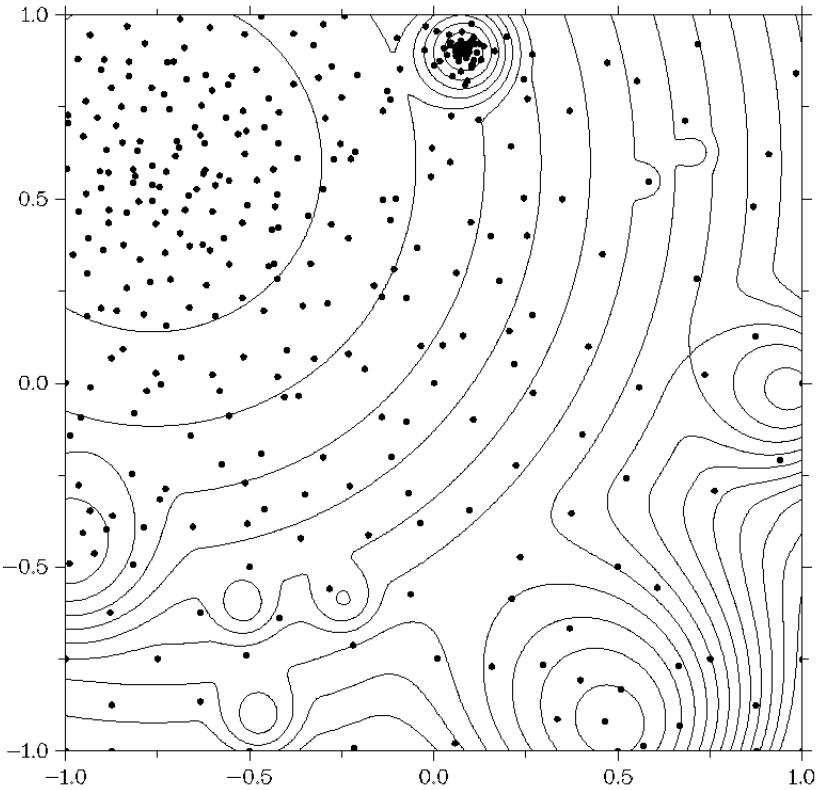
\includegraphics[width=0.45\textwidth]{isolines.png}
		\caption{Решение двумерной задачи}\label{fig:isolines}
\end{figure}
\par
Для примера на рис. \ref{fig:isolines} приведены линии уровня двумерной функции, порождаемой GKLS-генератором. Темные точки соответствуют 464 испытаниям, потребовавшимся для решения данной задачи с точностью 0.01 по координате; при этом число итераций составило 58 (на каждой итерации проводилось 8 испытаний). Линии уровня наглядно демонстрируют многоэкстремальность задачи, а расположение точек --- неравномерное покрытие, сгущающееся только в районе глобального минимума.
\par
Ниже приведены результаты численного сравнения трех последовательных алгоритмов --- DIRECT \cite{zilinsk}, DIRECT\(l\)  \cite{sergKvaDiaPaper} и алгоритма глобального поиска (АГП) (результаты работы первых двух алгоритмов приводятся по работе \cite{jonesLipOpt}). Численное сравнение проводилось на классах функций Simple и Hard размерности 4 и 5 из \cite{jonesLipOpt}. Глобальный минимум \(y^*\) считался найденным, если алгоритм генерировал точку испытания \(y_k\) в \(\delta\)-окрестности глобального минимума, т.е. \(\Vert y_k-y^*\Vert\leqslant\delta\). При этом размер окрестности выбирался (в соответствии с \cite{jonesLipOpt}) как \(\delta=\Vert b-a\Vert \sqrt[N]{\Delta}\), здесь \(N\) --- размерность решаемой задачи, \(a\) и \(b\) --- границы области поиска \(D\), параметр \(\Delta=10^{-6}\) при \(N=4\) и \(\Delta=10^{-7}\) при \(N=5\). При использовании метода АГП для класса Simple выбирался параметр \(r=4.5\), для класса Hard --- \(r=5.6\); параметр построения кривой Пеано был фиксированный \(m=10\). Максимально допустимое число итераций составляло \(K_{max} = 1 000 000\).
\par
В таблице 1 отражено среднее число итераций \(k_{av}\), которые выполнил метод при решении серии задач из данных классов. Символ «>» отражает ситуацию, когда не все задачи класса были решены каким-либо методом. Это означает, что алгоритм был остановлен по причине достижения максимально допустимого числа итераций \(K_{max}\). В этом случае значение \(K_{max}=1 000 000\) использовалось при вычислении среднего значения числа итераций \(k_{av}\), что соответствует нижней оценке этого среднего значения. Количество нерешенных задач указано в скобках.
\begin{table}
    \centering
    \begin{tabular}{|c|p{3cm}|c|c|c|}
    \hline
    \(N\) & Класс функций & DIRECT & DIRECT\(l\) & АГП \\ \hline
    4 & Simple & >47282 (4) & 18983 & 11953\\ \cline{2-5}
      & Hard & >95708 (7) & 68754 & 68754\\ \hline
    5 & Simple & >16057 (1) & 16758 & 15920\\ \cline{2-5}
      & Hard & >217215 (16) & >269064 (4) & >148342 (4)\\ \hline
    \end{tabular}
    \caption{Среднее число итераций}
    \label{table:average_iters}
\end{table}
\par
Как видно из таблицы \ref{table:average_iters}, АГП превосходит методы DIRECT и DIRECT\(l\) на всех классах задач по среднему числу итераций. При этом в классе 5-Hard каждый из методов решил не все задачи: DIRECT не решил 16 задач, DIRECT\(l\) и АГП – по 4 задачи.
\subsection{Задачи с трудоемким критерием}
Вначале приведем результаты экспериментов, которые соответствуют задачам с большим временем проведения одного поискового испытания. Оценим ускорение параллельного алгоритм глобального поиска (ПАГП), реализованного на CPU, в зависимости от использованного количества ядер \(p\). В таблицах \ref{table:time_speedUp_cpu} и \ref{table:iterations_speedUp_cpu} приведено ускорение по времени \(S(p)\) и по итерациям \(s(p)\). Ускорение вычислено относительно однопоточного запуска.
\begin{table}
    \centering
    \begin{tabular}{|c|c|c|c|c|}
    \hline
    \(p\) & \multicolumn{2}{|c|}{\(N=4\)} & \multicolumn{2}{|c|}{\(N=5\)}\\ \cline{2-5}
    & Simple & Hard & Simple & Hard \\ \hline
    2 & 2.45 & 2.20 & 1.15 & 1.32\\ \hline
	4 & 4.66 & 3.90 & 2.82 & 2.59\\ \hline
	8 & 7.13 & 7.35 & 3.47 & 5.34\\ \hline
    \end{tabular}
    \caption{Ускорение по времени \(S(p)\) на CPU}
    \label{table:time_speedUp_cpu}
\end{table}
\begin{table}
    \centering
    \begin{tabular}{|c|c|c|c|c|}
    \hline
    \(p\) & \multicolumn{2}{|c|}{\(N=4\)} & \multicolumn{2}{|c|}{\(N=5\)}\\ \cline{2-5}
    & Simple & Hard & Simple & Hard \\ \hline
	2 & 2.51 & 2.26 & 1.19 & 1.36\\ \hline
	4 & 5.04 & 4.23 & 3.06 & 2.86\\ \hline
	8 & 8.58 & 8.79 & 4.22 & 6.56\\ \hline
    \end{tabular}
    \caption{Ускорение по итерациям \(s(p)\) на CPU}
    \label{table:iterations_speedUp_cpu}
\end{table}
\par
Результаты экспериментов показывают значительное ускорение ПАГП при использовании CPU. Лучшие результаты получены при использовании всех ядер процессора.
\par
Далее изложим результаты экспериментов, проведенных с использованием Intel Xeon Phi. Вначале рассмотрим эксперименты на одном Xeon Phi в режиме Offload. Варьировалось количество потоков на сопроцессоре, все остальные параметры совпадают с предыдущими запусками. Приведено (таблицы \ref{table:time_speedUp_phi} и \ref{table:iterations_speedUp_phi}) ускорение относительно восьмипоточного запуска на центральном процессоре.
\begin{table}
    \centering
    \begin{tabular}{|c|c|c|c|c|}
    \hline
    \(p\) & \multicolumn{2}{|c|}{\(N=4\)} & \multicolumn{2}{|c|}{\(N=5\)}\\ \cline{2-5}
    & Simple & Hard & Simple & Hard \\ \hline
	60 & 0.54 & 1.02 & 1.07 & 1.61\\ \hline
	120 & 0.55 & 1.17 & 1.05 & 2.61\\ \hline
	240 & 0.51 & 1.06 & 1.07 & 4.17\\ \hline
    \end{tabular}
    \caption{Ускорение по времени \(S(p)\) на Phi}
    \label{table:time_speedUp_phi}
\end{table}
\begin{table}
    \centering
    \begin{tabular}{|c|c|c|c|c|}
    \hline
    \(p\) & \multicolumn{2}{|c|}{\(N=4\)} & \multicolumn{2}{|c|}{\(N=5\)}\\ \cline{2-5}
    & Simple & Hard & Simple & Hard \\ \hline
	60 & 8.13 & 7.32 & 9.87 & 6.55 \\ \hline
	120 & 16.33 & 15.82 & 15.15 & 17.31 \\ \hline
	240 & 33.07 & 27.79 & 38.80 & 59.31 \\ \hline
    \end{tabular}
    \caption{Ускорение по итерациям \(s(p)\) на Phi}
    \label{table:iterations_speedUp_phi}
\end{table}
\par
Результаты экспериментов показывают, что только на классе Simple при \(N=4\) реализация на Xeon Phi медленнее, чем CPU реализация, на классе Hard при \(N=4\) и на классе Simple при \(N=5\) версии для Xeon Phi и CPU демонстрирует примерно равную эффективность, а на классе Hard при \(N=5\) версия для Xeon Phi существенно превосходит CPU-реализацию. Наибольшее преимущество реализация для Xeon Phi показывает при 120 потоках для четырехмерных задач и при 240 потоках для пятимерных. При этом на всех классах наблюдается значительное ускорение по итерациям, а также практически линейная масштабируемость от числа потоков.
\par
Далее рассмотрим эксперименты с запуском сопроцессора в режиме MPI. Число уровней вложенности разбиваемой задачи равно двум. Число процессов, запущенных на сопроцессоре, –-- 30 (таблицы \ref{table:time_speedUp_phi_30mpi} и \ref{table:iterations_speedUp_phi_30mpi}) и 60(таблицы \ref{table:time_speedUp_phi_60mpi} и \ref{table:iterations_speedUp_phi_60mpi}), что соответствует ситуации, когда у корня дерева имеется соответственно 30 и 60 потомков. Процессы, работающие на сопроцессоре, использовали OpenMP для параллельного вычисления значений функции. Ускорение приведено относительно восьмипоточного запуска на CPU.
\begin{table}
    \centering
    \begin{tabular}{|c|c|c|c|c|}
    \hline
    \(p\) & \multicolumn{2}{|c|}{\(N=4\)} & \multicolumn{2}{|c|}{\(N=5\)}\\ \cline{2-5}
    & Simple & Hard & Simple & Hard \\ \hline
	4 & 3,18 & 5,14 & 5,15 & 14,65 \\ \hline
	8 & 3,53 & 1,49 & 3,35 & 10,49 \\ \hline
	16 & 1,09 & 2,77 & 4,61 & 14,36 \\ \hline
    \end{tabular}
    \caption{Ускорение по времени \(S(p)\) на Phi, 30 MPI процессов}
    \label{table:time_speedUp_phi_30mpi}
\end{table}
\begin{table}
    \centering
    \begin{tabular}{|c|c|c|c|c|}
    \hline
    \(p\) & \multicolumn{2}{|c|}{\(N=4\)} & \multicolumn{2}{|c|}{\(N=5\)}\\ \cline{2-5}
	4 & 11,19 & 19,19 & 9,27 & 27,38 \\ \hline
	8 & 13,97 & 3,63 & 8,24 & 23,85 \\ \hline
	16 & 1,29 & 3,56 & 8,28 & 22,12 \\ \hline
	\end{tabular}
    \caption{Ускорение по итерациям \(s(p)\) на Phi, 30 MPI процессов}
    \label{table:iterations_speedUp_phi_30mpi}
\end{table}
\begin{table}
    \centering
    \begin{tabular}{|c|c|c|c|c|}
    \hline
    \(p\) & \multicolumn{2}{|c|}{\(N=4\)} & \multicolumn{2}{|c|}{\(N=5\)}\\ \cline{2-5}
    & Simple & Hard & Simple & Hard \\ \hline
	4 & 2,76 & 3,20 & 4,19 & 16,56 \\ \hline
	8 & 3,05 & 7,73 & 4,08 & 14,87 \\ \hline
	16 & 0,89 & 5,21 & 2,72 & 13,05 \\ \hline
    \end{tabular}
    \caption{Ускорение по времени \(S(p)\) на Phi, 60 MPI процессов}
    \label{table:time_speedUp_phi_60mpi}
\end{table}
\begin{table}
    \centering
    \begin{tabular}{|c|c|c|c|c|}
    \hline
    \(p\) & \multicolumn{2}{|c|}{\(N=4\)} & \multicolumn{2}{|c|}{\(N=5\)}\\ \cline{2-5}
	4 & 10,36 & 3,34 & 6,01 & 26,04 \\ \hline
	8 & 9,04 & 28,81 & 7,68 & 25,02 \\ \hline
	16 & 1,27 & 28,66 & 7,19 & 30,38 \\ \hline
	\end{tabular}
    \caption{Ускорение по итерациям \(s(p)\) на Phi, 60 MPI процессов}
    \label{table:iterations_speedUp_phi_60mpi}
\end{table}
\par
Результаты экспериментов показывают, что запуск в режиме MPI значительно превосходит Offload режим по времени работы, однако проигрывает по числу итераций. Лучшие результаты для простого класса задач наблюдаются при использовании 30 процессов на сопроцессоре, а для сложного класса, при 60 процессах. Таким образом, можно сделать вывод, что задачи с большим временем работы, для которых важно число итераций метода оптимизации, лучше использовать запуск в режиме Offload, а для более быстро решаемых задач, лучше подходит режим MPI. 
\subsection{Задачи с легко вычисляемым критерием}
Рассмотрим теперь решение задач, в которых поисковые испытания проводятся быстро. Вначале приведем результаты OpenMP версии. В таблице \ref{table:time_speedUp_cpu_2} приведено ускорение относительно однопоточного запуска.
\begin{table}
    \centering
    \begin{tabular}{|c|c|c|c|c|}
    \hline
    \(p\) & \multicolumn{2}{|c|}{\(N=4\)} & \multicolumn{2}{|c|}{\(N=5\)}\\ \cline{2-5}
    & Simple & Hard & Simple & Hard \\ \hline
	2 & 1,09 & 1,09 & 0,56 & 0,57 \\ \hline
	4 & 1,10 & 1,06 & 0,74 & 0,66 \\ \hline
	8 & 0,90 & 1,11 & 0,45 & 1,77 \\ \hline
	16 & 0,66 & 0,92 & 0,76 & 0,66 \\ \hline
	32 & 0,29 & 0,38 & 0,22 & 0,55 \\ \hline
    \end{tabular}
    \caption{Ускорение по времени \(S(p)\) на CPU}
    \label{table:time_speedUp_cpu_2}
\end{table}
\par
Эксперименты показывают незначительное ускорение, а во многих случаях – и замедление при вычислениях только на центральном процессоре.
\par
Далее рассмотрим ускорение при использовании Xeon Phi в режиме MPI. Результаты приведены относительно однопоточного запуска на CPU. В таблице \ref{table:time_speedUp_phi_30mpi_easy} приведено ускорение по времени \(S(p)\) для запуска 30 процессов на Xeon Phi, в таблице \ref{table:time_speedUp_phi_60mpi_easy} для 60 процессов.
\begin{table}
    \centering
    \begin{tabular}{|c|c|c|c|c|}
    \hline
    \(p\) & \multicolumn{2}{|c|}{\(N=4\)} & \multicolumn{2}{|c|}{\(N=5\)}\\ \cline{2-5}
    & Simple & Hard & Simple & Hard \\ \hline
	1 & 0,35 & 2,28 & 0,37 & 1,92 \\ \hline
	2 & 0,94 & 1,95 & 0,39 & 1,23 \\ \hline
	4 & 1,23 & 0,43 & 0,54 & 2,63 \\ \hline
	8 & 0,85 & 0,56 & 0,40 & 1,53 \\ \hline
	\end{tabular}
    \caption{Ускорение по времени \(S(p)\) на Phi, 30 MPI процессов}
    \label{table:time_speedUp_phi_30mpi_easy}
\end{table}
\begin{table}
    \centering
    \begin{tabular}{|c|c|c|c|c|}
    \hline
    \(p\) & \multicolumn{2}{|c|}{\(N=4\)} & \multicolumn{2}{|c|}{\(N=5\)}\\ \cline{2-5}
    & Simple & Hard & Simple & Hard \\ \hline
	1 & 0,59 & 2,56 & 1,22 & 3,30 \\ \hline
	2 & 0,89 & 0,87 & 1,29 & 2,76 \\ \hline
	4 & 1,09 & 1,03 & 0,38 & 5,32 \\ \hline
	8 & 0,70 & 0,78 & 0,69 & 2,19 \\ \hline
	\end{tabular}
    \caption{Ускорение по времени \(S(p)\) на Phi, 60 MPI процессов}
    \label{table:time_speedUp_phi_60mpi_easy}
\end{table}
\par
Результаты экспериментов показывают ускорение на Xeon Phi, превосходящее ускорение на центральном процессоре. Лучшие результаты получены при использовании 30 процессов на Xeon Phi только для простых четырехмерных задач, все остальные задачи лучше всего решаются при использовании 60 процессов.
\par
Теперь перейдем к эксперименту с шестимерными задачами простого класса. При решении шестимерной задачи с использованием одного процесса (вложенные подзадачи отсутствуют) и сохранением точности построения развертки \(m=10\) требуется использовать числа с плавающей запятой расширенной точности, что ведет к значительному увеличению времени работы алгоритма. При этом в случае использования хотя бы одного уровня вложенных подзадач, задачи на каждом уровне будут решаться без подключения расширенной точности, что обеспечивает дополнительное преимущество блочной многошаговой схемы.
\par
Рассмотрим результаты эксперимента с использованием Xeon Phi в режиме MPI, таблица \ref{table:time_speedUp_phi_2}. Число уровней вложенности разбиваемой задачи равно двум. Приведены результаты экспериментов для разбиений 3:3 (три переменных на первом уровне, три – на втором) и 4:2 (4 переменных на первом уровне, две – на втором). Число процессов, запущенных на сопроцессоре равно 30 и 60, что соответствует тому, что у корня дерева имеется соответственно 30 и 60 потомков. Процессы, работающие на Xeon Phi, использовали OpenMP для параллельного вычисления значений функции. Ускорение приведено относительно однопоточного запуска на CPU.
\begin{table}
    \centering
    \begin{tabular}{|c|c|c|c|c|}
    \hline
    \(p\) & \multicolumn{2}{|c|}{30 процессов} & \multicolumn{2}{|c|}{60 процессов}\\ \cline{2-5}
	& 3:3 & 4:2 & 3:3 & 4:2 \\ \hline
	2 & 7,30 & 9,87 & 17,68 & 18,21 \\ \hline
	4 & 5,99 & 8,18 & 6,60 & 13,57 \\ \hline
	8 & 3,14 & 12,74 & 5,92 & 25,58 \\ \hline
	16 & 3,54 & 7,61 & 4,87 & 11,33 \\ \hline
	32 & 3,41 & 6,85 & 3,73 & 6,50 \\ \hline
\end{tabular}
    \caption{Ускорение по времени \(S(p)\) на Phi}
    \label{table:time_speedUp_phi_2}
\end{table}
\par
Результаты экспериментов показывают значительное ускорение запуска на сопроцессоре по сравнению с запуском только на центральном процессоре. Лучшее ускорение наблюдается при шестидесяти MPI процессах на Xeon Phi по 8 потоков на каждый процесс, время работы в 25 раз меньше, чем решение задачи только на центральном процессоре.
